%%%%% --------------------------------------------------------------------------------
%%
%%                               Document Template
%%
%%%%% --------------------------------------------------------------------------------
%% FORKED GITHUB PROJECT:
%% MODIFIED BY SEBASTIEN BLANCHET JUNE 2017
%%%%% --------------------------------------------------------------------------------
%%
%%%%************************ Document Class Declaration ******************************
%%
\documentclass[singlesided]{Style/uwaterloothesis}% thesis template of University of Waterloo
%% Multiple optional arguments:
%% [<singlesided|doublesided|printcopy>] % single-sided, double-sided, or print layout
%% [draftversion] % show draft version information, default is no show
%% [standard options for book class]
%%%%% --------------------------------------------------------------------------------
%%
%%%%************************* Command Define and Settings ****************************
%%
\usepackage[list, table]{Style/commons}% common settings
%% usage: \usepackage[option1,option2,...,optionN]{commons}
%% Multiple optional arguments:
%% [<numbered|authoryear|alpha>] % citation and reference style
%% <numbered>: textual: Jones [1]; parenthetical: [1]. default style
%% <authoryear>: textual: Jones (1995); parenthetical: (Jones, 1995)
%% <alpha>: textual: not available; parenthetical: [Jon95]
%% [myhdr] % one available header and footer style, will enable fancyhdr
%% [lscape] % provide landscape layout environment
%% [geometry] % configure page layout by geometry package
%% [list] % enable enhanced list environments, useful for Algorithm and Coding
%% [color] % enable color package to use color, default package is xcolor
%% [background] % enable page background, will auto enable color package
%% [tikz] % enable tikz for complex diagrams, will auto enbale color package
%% [table] % enable a t able package for complex tables, default is ctable
%% [math] % enable some extra math packages


%% Added packages
\usepackage{Style/custom}% user defined commands
%% For multi line equations
\usepackage{mathtools}
%\usepackage{amsmath}
%% For paragraph indentation, removes all indentation
\usepackage{parskip}
% for code import in appendix
\usepackage{listings}
% for proper figures placement
\usepackage{float}
% for properly formated section begining
\usepackage[compact]{titlesec}
\titleformat{\chapter}{\bf\normalfont\large}{\bf\thechapter.}{18pt}{\bf\large}
% default spacing for header is 50 pt before, 40 pt after
\titlespacing*{\chapter}{0pt}{0pt}{12pt}
% for appendices
\usepackage[toc,page]{appendix}
% for pdf import
\usepackage{pdfpages}
% matrix
\usepackage{amsmath}

% remove page break
\usepackage{etoolbox}
\makeatletter
\patchcmd{\chapter}{\if@openright\cleardoublepage\else\clearpage\fi}{}{}{}
\makeatother



%%%%% --------------------------------------------------------------------------------
%%
%%%%******************************** Content *****************************************
%%
\begin{document}
%%
%%%%% --------------------------------------------------------------------------------


%%%%******************************** Frontmatter *************************************
%%
%% Frontmatter of Title page, Table of contents, Preface chapter.
\frontmatter
%%
%% >>> Frontpages
%%
%%
%% >>> Title Page
%%
%%\LaTeX{} is Latex printed in right way
%% Define new commands (add space after defined names0
\newcommand{\Term}{4A }
\newcommand{\Seb}{Sebastien Blanchet }
\newcommand{\DelivName}{Assignment 2}
\newcommand{\ReportTitle}{}
\newcommand{\Prof}{Mihaela Vlasea, PhD}
\newcommand{\CourseName}{ME 561: Fluid Powder Control System}

%% Define command variable names
\title[\DelivName]{\DelivName}% \title[short title for headers]{Long title of thesis}
\author{\Seb}
\preparedfor{\Prof}
\preparedcity{\CourseName}
\discipline{\Term Mechanical Engineering}
\maketitle

%%
%%% >>> List of Content
%%
%% Set TOC to record subsections
\setcounter{tocdepth}{3}
\setcounter{secnumdepth}{3}
%% TOC LOF LOT
%\intotoc{\contentsname}% add a corresponding item to the contents table and bookmark
%\tableofcontents% contents catalog
%\intotoc{\listfigurename}% add a corresponding item to the contents table and bookmark
%\listoffigures% figures catalog
%\intotoc{\listtablename}% add a corresponding item to the contents table and bookmark
%\listoftables% tables catalog

%%%%% --------------------------------------------------------------------------------

%%%%******************************** Mainmatter **************************************
%%
%% Main topics.
\mainmatter
%%
%%% >>> Main Contents
%%
%%
%%% ++++++++++++++++++++++++++++++++++++++++++++++++++++++++++++++++++++++++++++++++++
%-----------------------------------------------------------------------------------------------------------------
%% Section 1
\chapter{Mass Actuator System}
\label{chap:q1}

The natural frequency $\omega_n$ of the mass actuator system in Figure~\ref{fig:q1} \cite{assign} below is of interest.

\begin{figure}[H]
	\centering
	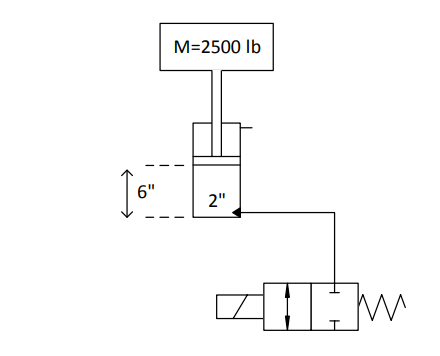
\includegraphics[scale=0.75]{q1}
	\caption{Question 1 circuit schematic.}
	\label{fig:q1}
\end{figure}

Constant parameters are listed in Table~\ref{tab:q1_param}. Furthermore, the following assumptions are made \cite{assign}.
\begin{itemize}
	\item De-energized directional valve
	\item Rigid cylinder walls
	\item No air content
\end{itemize}

\begin{table}[H]
	\centering
	\caption{Given parameters.}
	\begin{tabular}{cccc}
		\toprule
		\textbf{Description} & \textbf{Symbol} & \textbf{Value } & \textbf{Unit} \\
		\midrule
		Mass                 & $m$             & 2500            & lbm           \\
		Stroke               & $l$             & 6               & in            \\
		Diameter             & $D$             & 2               & in            \\
		Bulk modulus         & $\beta$         & 260000          & psi           \\
		\bottomrule    
	\end{tabular}
	\label{tab:q1_param}
\end{table}

To find $\omega_n$, the system's dynamics must be derived. This is done with the hydraulic system's equivalent mass spring damper model. Note that because there is no air content  $b=0$, however it will be kept for the derivation. Applying Newton's second law to the free body diagram in Figure~\ref{fig:q1_fbd} will yield the final result in \ref{eq:q1_newt}.

\begin{figure}[H]
	\centering
	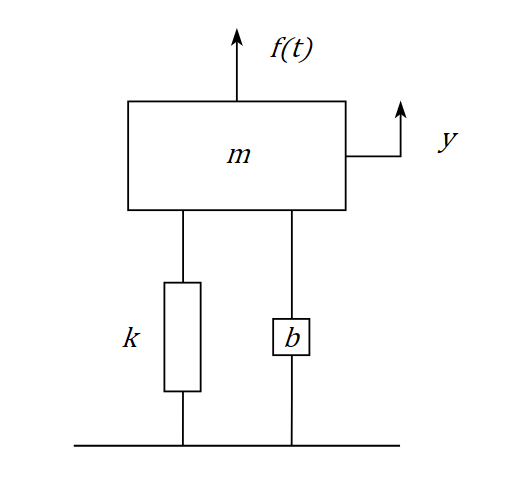
\includegraphics[scale=0.75]{q1_fbd}
	\caption{Free body diagram.}
	\label{fig:q1_fbd}
\end{figure}

\begin{equation}
	\label{eq:q1_newt}
	m \ddot{y} = f(t) - b\dot{y} - k y
\end{equation}

Taking the Laplace transform $\mathcal{L}$ of \ref{eq:q1_newt} with zero initial conditions and rearranging to get in standard plant model form \ref{eq:q1_tfactual}.

\begin{equation*}
	ms^2 Y(s) + b s Y(s) + k Y(s) = F(s)
\end{equation*}

\begin{equation}
	\label{eq:q1_tfactual}
	P(s) = \frac{Y(s)}{F(s)} = \frac{\frac{1}{m}}{s^2 + \frac{b}{m}s + \frac{k}{m}}
\end{equation}

From this, the natural frequency can be extrapolated from the ideal second order transfer function $P(s)$ \ref{eq:q1_tfideal}.
\begin{equation}
	\label{eq:q1_tfideal}
	P(s)= \frac{\omega_n^2}{s^2+2\zeta\omega_n s + \omega_n^2}
\end{equation}

Comparing like coefficients yields a final expression for $\omega_n$ \ref{eq:q1_wn}.
\begin{equation}
	\label{eq:q1_wn}	
	\omega_n = \sqrt{\frac{386k}{m}}	
\end{equation}

Note that the above units of $k$ are equivalent to [lbf/in] and 1 [lbf] = 32.174 [lbm $\cdot$ ft/$\Unit{s^2}$] therefore 1 [lbf] = 386 [lbm $\cdot$ in/$\Unit{s^2}$], which is the added factor. As a result \ref{eq:q1_wn} yields a frequency in [rad/s].\\

The mass $m$ is given in Table~\ref{tab:q1_param} , therefore it is required to find the equivalent stiffness constant $k$. This is done with the bulk modulus equation $\beta$ as per \ref{eq:q1_beta}.
\begin{equation}
	\label{eq:q1_beta}
	\beta = - \frac{\Delta p V_0}{\Delta V}	
\end{equation}

Realizing that $V_0 = AL$ and $\Delta V = Ax$, rearranging \ref{eq:q1_beta} for $\Delta p$ and comparing with well known $p =F/A$ relation yields \ref{eq:q1_f}.

\begin{equation*}
	\Delta p = \beta \ \frac{y}{l} = \frac{F}{A}
\end{equation*}

\begin{equation}
	\label{eq:q1_f}
	\Rightarrow F = \frac{A\beta}{l}y 	
\end{equation}

Knowing that $F = ky$, comparing the result of \ref{eq:q1_f} yields the final relation for the equivalent stiffness $k$ in [lbf/in]. 

\begin{equation}
	\label{eq:q1_k}
	k = \frac{A\beta}{l} 	
\end{equation}

Applying the above equations with parameters from \cite{assign} yields the final results in Table~\ref{tab:q1_ans}. Note all calculations in foregoing sections performed with \cite{excel}.
 
\begin{table}[H]
	\centering
	\caption{Calculated values.}
	\begin{tabular}{cccc}
		\toprule    
		\textbf{Description} & \textbf{Symbol} & \textbf{Value } & \textbf{Unit} \\
		\midrule
		Area                 & $A$             & 3.142           & $\Unit{in^2}$ \\
		Volume               & $\forall_0$     & 18.850          & $\Unit{in^3}$ \\
		Stiffness            & $k$             & 1.361E+05       & lbf/in        \\
		Natural frequency    & $\omega_n$      & 144.981         & rad/s         \\
		\bottomrule    
	\end{tabular}
	\label{tab:q1_ans}
\end{table}

The natural frequency of the system is \textbf{144.981 [rad/s]} or \textbf{23.074 [Hz]}.

%-----------------------------------------------------------------------------------------------------------------
%% Section 2
\chapter{Accumulator System}
\label{chap:q2}

The following circuit schemic for an accumulator system is given in Figure~\ref{fig:q2} below \cite{assign}.

\begin{figure}[H]
	\centering
	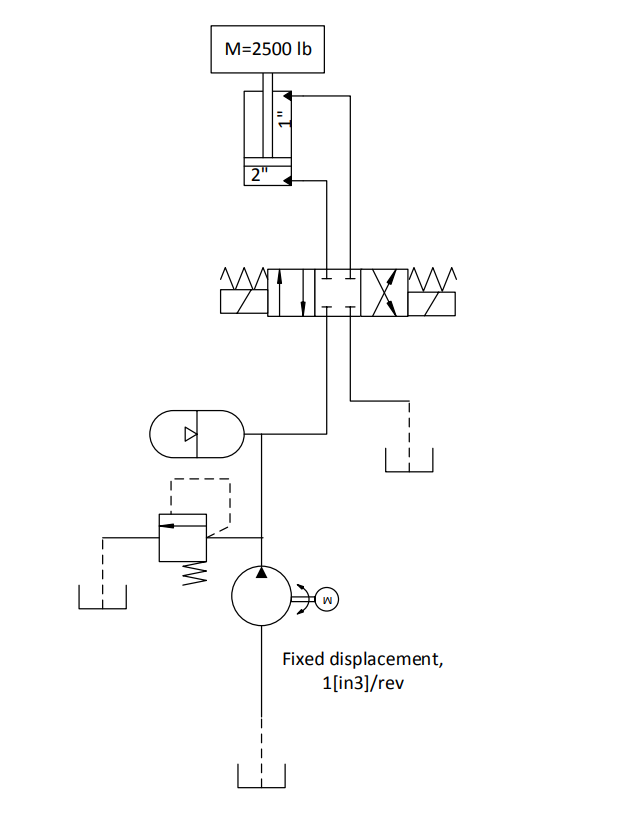
\includegraphics[scale=0.75]{q2}
	\caption{Question 2 circuit schematic.}
	\label{fig:q2}
\end{figure}

Constant parameters are listed in Table~\ref{tab:q2_param} \cite{assign}. 
\begin{table}[H]
	\centering
	\caption{Question 2 constant parameters.}
	\begin{tabular}{cccc}
		\toprule
		\textbf{Description}            & \textbf{Symbol} & \textbf{Value } & \textbf{Unit}     \\
		\midrule
		Piston diameter                 & $D_P$           & 2               & in                \\
		Rod diameter                    & $D_R$           & 1               & in                \\
		Stroke length                   & $L$             & 10              & in                \\
		Weight of mass                  & $W$             & 2500            & lbf               \\
		Actuator speed                  & $v$             & 45              & in/s              \\
		Relief valve opening pressure   & $p_{RV}$        & 230             & bar               \\
		Accumulator pre-charge pressure & $p_A$           & 1800            & psig              \\
		Pump speed                      & $N$             & 1700            & RPM               \\
		Pump displacement volume        & $V_D$           & 1               & $\Unit{in^3/rev}$ \\
		Pump volumetric efficiency      & $\eta_V$        & 100             & \%                \\
		\bottomrule    
	\end{tabular}
	\label{tab:q2_param}%
\end{table}%

Again, the assumptions made for this question are listed as follows as per \cite{assign}.
\begin{itemize}
	\item Actuator initially fully retracted
	\item Positive displacement pump
	\item Return line pressure $p_2$ is 0 psi (gauge)
	\item Accumulator air is an ideal gas $\Rightarrow \gamma=1.4$ 
	\item Accumulator effective volume when no oil in it
	\item No length losses
\end{itemize}

\section{Hydraulic Pump Pressure}

The pump pressure $p_P$ is of interest. To find this value, the required piston end flow rate $Q_1$ is calculated with \ref{eq:q2_q1}. Note that the piston end area is defined as $A_1 = \tfrac{\pi}{4} D_P^2$.

\begin{equation}
	\label{eq:q2_q1}
	Q_1 = A_1 v
\end{equation}

Using this flow rate, the pressure loss $\Delta p_1$ across the valve on the piston side is defined as \ref{eq:q2_ploss} \cite{assign}.

\begin{equation}
	\label{eq:q2_ploss}
	\Delta p_1 = 50 \left( \frac{Q_1}{100} \right)^2
\end{equation}

Note that the above equation is for $p$ in [bar] and $Q$ in [$\Unit{in^3/s}$].\\

The required hydraulic pressure at the pump outlet $p_P$ is simply the required piston pressure plus the loss \ref{eq:q2_ppump}.
\begin{equation}
	\label{eq:q2_ppump}
	p_P = p_1 + \Delta p
\end{equation}

Hence, it is first required to find the pressure exerted on the piston $p_1$. Knowing that $F=pA$, a force balance in the $y$ direction ($\uparrow^+  \Sigma F_y = 0$) yields the final relation \ref{eq:q2_p1}. Note the rod end cylinder area is defined as $A_2 = \tfrac{\pi}{4}\left( D_P^2 - D_R^2 \right)$.

\begin{equation*}
	p_1 A_1 = p_2 A_2 + W
\end{equation*}

\begin{equation}
	\label{eq:q2_p1}
	p_1 = \frac{1}{14.5} \left(\frac{p_2 A_2 + W}{A_1} \right)
\end{equation}
A factor of 14.5 is added since $p_{\Unit{bar}} = 14.5 \cdot p_{\Unit{psi}}$.\\

From above, $p_2$ is still unknown. Since the return line pressure is 0 [psi], the pressure on the rod end is simply pressure loss across that side of the valve $\Delta p_2$ as per \ref{eq:q2_ploss2} \cite{assign}.

\begin{equation}
	\label{eq:q2_ploss2}
	\Delta p_2 = 50 \left( \frac{Q_2}{100} \right)^2
\end{equation}

Therefore, $Q_2$ is defined as \ref{eq:q2_q2}.
\begin{equation}
	\label{eq:q2_q2}
	Q_2 = \frac{V_{D2}}{t} = \frac{A_2 L}{t}
\end{equation}

Where the cycle time is \ref{eq:q2_tcyl}.

\begin{equation}
	\label{eq:q2_tcyl}
	t = \frac{V_{D1}}{Q_1} = \frac{A_1 L}{Q_1} 
\end{equation}

\pagebreak

Following the aforementioned procedure yields results in Table~\ref{tab:q2a_ans} below.
\begin{table}[H]
	\centering
	\caption{Question 2, part A results.}
	\begin{tabular}{cccc}
		\toprule
		\textbf{Description}          & \textbf{Symbol} & \textbf{Value } & \textbf{Unit}   \\
		\midrule
		Piston end area               & $A_1$           & 3.142           & $\Unit{in^2}$   \\
		Rod end area                  & $A_2$           & 2.356           & $\Unit{in^2}$   \\
		Required piston end flow rate & $Q_1$           & 141.372         & $\Unit{in^3/s}$ \\
		Rod end flow rate             & $Q_2$           & 106.029			& $\Unit{in^3/s}$ \\
		Cycle time                    & $t$             & 0.222           & s               \\
		Pressure loss per valve land  & $\Delta p_1$    & 99.930          & bar             \\
		Pressure loss rod end         & $\Delta p_2$    & 56.210         & bar             \\
		Piston end pressure           & $p_1$           & 97.025          & bar             \\
		Pump pressure                 & $p_P$           & 196.955         & bar             \\
		\bottomrule
	\end{tabular}
	\label{tab:q2a_ans}
\end{table}%

Hence in can be concluded that a pump pressure of \textbf{196.955 [bar]} or \textbf{2857 [psi]} is required.

\pagebreak

\section{Accumulator Effective Volume}

Assuming that the accumulator is adiabatic due to the short cycle time \cite{notes}, the accumulator's effect gas volume $V_1$ is calculated with \ref{eq:q2_acum}.

\begin{equation}
	\label{eq:q2_acum}
	V_1 = \frac{\Delta V}{\left( \frac{p_1}{p_2} \right)^{\frac{1}{\gamma}} -\left( \frac{p_1}{p_3}\right)^{\frac{1}{\gamma}}}
\end{equation}

Where $p_1 \equiv$ accumulator's pre charged pressure (or $p_A$ see Table \ref{tab:q2_param}), $p_2 \equiv$ pump pressure (or $p_P$ see Table \ref{tab:q2a_ans}) and $p_3 \equiv$ maximum pressure (or $p_{RV}$ see Table \ref{tab:q2_param}).\\


To find $\Delta V$, must find the specified area under the curve in Figure~\ref{fig:q2_accum}, resulting in  \ref{eq:q2_delv}.
\begin{figure}[H]
	\centering
	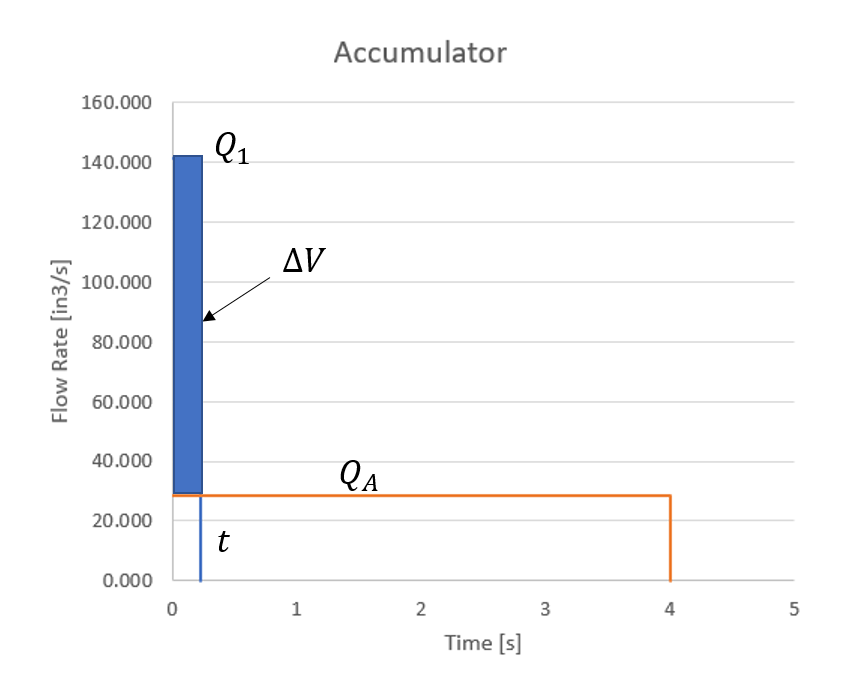
\includegraphics[scale=0.5]{q2_accum}
	\caption{Question 2 flow rate plot.}
	\label{fig:q2_accum}
\end{figure}

\begin{equation}
	\label{eq:q2_delv}
	\Delta V = \left( Q_1 - Q_A \right)t
\end{equation}

Where $Q_A$ is the actual pump flow rate and $t$ the cycle time from Table~\ref{tab:q2a_ans}. Recall that $\eta_V = Q_A/Q_T \therefore Q_T = Q_A \because \eta_V = 100 \% $. From this the actual pump flow rate is calculated as \ref{eq:q2_qa}.

\begin{equation}
	\label{eq:q2_qa}
	Q_A = \frac{1}{60} V_D N
\end{equation}

Note, a factor of 1/60 is added for $[\Unit{in^3/min}] \rightarrow [\Unit{in^3/s}]$.\\


Applying all previous equations will yield the final results in Table~\ref{tab:q2c_ans}.
\begin{table}[H]
	\centering
	\caption{Question 2, part B results.}
	\begin{tabular}{cccc}
		\toprule
		\textbf{Description}             & \textbf{Symbol} & \textbf{Value } & \textbf{Unit}   \\
		\midrule
		Pre charge pressure              & $p_1$           & 125.083         & bar             \\
		Operating pressure               & $p_2$           & 196.955         & bar             \\
		Maximum pressure                 & $p_3$           & 230.000         & bar             \\
		Actual pump flow rate            & $Q_A$           & 28.333          & $\Unit{in^3/s}$ \\
		Change in volume                 & $\Delta V$      & 25.120          & $\Unit{in^3}$   \\
		Accumulator effective gas volume & $V_1$           & 331.271          & $\Unit{in^3}$   \\
		\bottomrule
	\end{tabular}
	\label{tab:q2c_ans}
\end{table}

The accumulator's effective gas volume is calculated as \textbf{331.271 [in\textsuperscript{3}]}.

%-----------------------------------------------------------------------------------------------------------------
%% Section 3
\chapter{Cascade Design}
\label{chap:q3}

A pneumatic cascade circuit is designed for the sequence in \ref{eq:q3_cd} \cite{assign}.

\begin{equation}
	\label{eq:q3_cd}
	A^+ B^+ B^- A^- C^+ C^- D^+ D^- 	
\end{equation}

The sequence must begin after a manual 3/2 start valve's is pressed momentarily. The following procedure is carried out.\\

\textit{1.} $n$ Groups are assigned such that there is no repeated letters \ref{eq:q3_groups} $\Rightarrow n=3$.

\begin{equation}
	\label{eq:q3_groups}
	\underbrace{A^+ B^+}_\text{I} \ \ \underbrace{B^- A^- C^+}_\text{II} \ \ \underbrace{C^- D^+}_\text{III} \ \ \underbrace{D^-}_\text{I}	
\end{equation}
\\

\textit{2.} Each cylinder ($A,B,C,D$) is assigned a 4/2 control valve and two 3/2 spring return limit values. This results in $n-1\Rightarrow 2$ cascade valves. The cascade valves are connected to the $n \Rightarrow 3$ pilot lines.\\

\textit{3.} Each respective limit valve's input is then connected to it's own group:
\begin{itemize}
	\item $D^- A^+ B^+\rightarrow$ I
	\item $B^- A^- C^+\rightarrow$ II
	\item $C^- D^+ \rightarrow$ III\\
\end{itemize}

\textit{4.}  The first letter of each group is then connected to its corresponding control valve:
\begin{itemize}
	\item $D^- \Rightarrow D_{Ret} \rightarrow$ I
	\item $B^- \Rightarrow B_{Ret} \rightarrow$ II
	\item $C^- \Rightarrow C_{Ret} \rightarrow$ III\\
\end{itemize}

\textit{5.}  The last letter of each group's limit valve output is then connected to next group's 5/2 cascade valve:
\begin{itemize}
	\item $B^+ \rightarrow$ I +1 $\rightarrow$ 2
	\item $C^+ \rightarrow$ II + 1 $\rightarrow$ 3
	\item $D^+ \rightarrow$ III + 1  $\rightarrow$ 1\\
\end{itemize}


\textit{6.} For the remainder of each values, the output on the corresponding limit valve is connected to the respective control valve input.
\begin{itemize}
	\item $A^+ \rightarrow B_{Ext}$
	\item $B^- \rightarrow A_{Ret}$
	\item $A^- \rightarrow C_{Ext}$
	\item $C^- \rightarrow D_{Ext}$\\
\end{itemize}

\textit{7.} The circuit is completed by connecting a 3/2 valve between $A_{Ext}$ and the input of $D^-$ limit valve.\\

Following the above listed steps, see the next page for the final cascade diagram.\\

\pagebreak
\includepdf[pages={1}]{cascade.pdf}
%%% ++++++++++++++++++++++++++++++++++++++++++++++++++++++++++++++++++++++++++++++++++



%%%%% --------------------------------------------------------------------------------
%%%%******************************* Backmatter ***************************************
%%
%% Matters of Bibliography, Glossary, Index.
\backmatter
%%
%%% >>> Bibliography
%%
%% Need to run bibtex in compiler 
\intotoc{\bibname}
%% Get IEEE reference style
\bibliographystyle{ieeetran}
\bibliography{Biblio/Refs}
%%

%%%%******************************** Appendix ****************************************
%%
\cleardoublepage
\backmatter
\chapter{Appendix}
\label{appendix:script}
\nopagebreak
\begin{scriptsize}
	\lstinputlisting[language=MATLAB]{"C:/Users/Sebastien/Documents/GitHub/ME561/A1/MATLAB/Main.m"}
\end{scriptsize}


%%%%%% --------------------------------------------------------------------------------

\end{document}
%%%%% --------------------------------------------------------------------------------
